\chapter{Spieren en gewrichten}\label{ch:g10:muscles-and-joints}

Een voetballer zet zijn voet neer, draait, en gaat neer terwijl hij zijn
knie vastgrijpt. De diagnose, een uur later: een gescheurde
\omterm{def:g10:muscles-and-joints:joint}{gewrichtsband}. Er is geen bot gebroken, geen spier bezweken; een reepje
weefsel van enkele centimeters, dat twee botten op één lijn moest
houden, is bezweken onder een draaibeweging waarvoor het nooit was
gebouwd. Om te begrijpen wat er scheurde, en waarom de knie maanden
nodig heeft om te herstellen, moeten we weten waaruit een \omterm{def:g10:muscles-and-joints:joint}{gewricht}
bestaat, hoe spieren eraan trekken, en welke krachten erdoorheen gaan
wanneer een lichaam van zeventig kilogram op één been landt.

\section{Het gewricht}

\begin{definition}[Gewricht]\label{def:g10:muscles-and-joints:joint}
Een \emph{gewricht}\index{gewricht} is de plaats waar twee botten elkaar
ontmoeten. In een beweeglijk gewricht zoals de knie, de heup, de
schouder of de elleboog zijn de uiteinden van de botten bedekt met een
laag glad \emph{kraakbeen}\index{kraakbeen} van enkele millimeters dik,
en omsloten door een gesloten zak, het \emph{gewrichtskapsel}, waarvan de
bekleding de \emph{gewrichtssmeer} afscheidt die de oppervlakken smeert.
Banden van taai weefsel, de
\emph{gewrichtsbanden}\index{gewrichtsband}, lopen van bot naar bot over
het gewricht heen en beperken de bewegingen tot de bedoelde. In de knie
liggen twee halvemaanvormige stukken kraakbeen, de \emph{menisci},
tussen de botten en verdelen zij de belasting.
\end{definition}

\begin{omfigure}
\begin{tikzpicture}
  \node[anchor=south west, inner sep=0] (img) at (0,0)
    {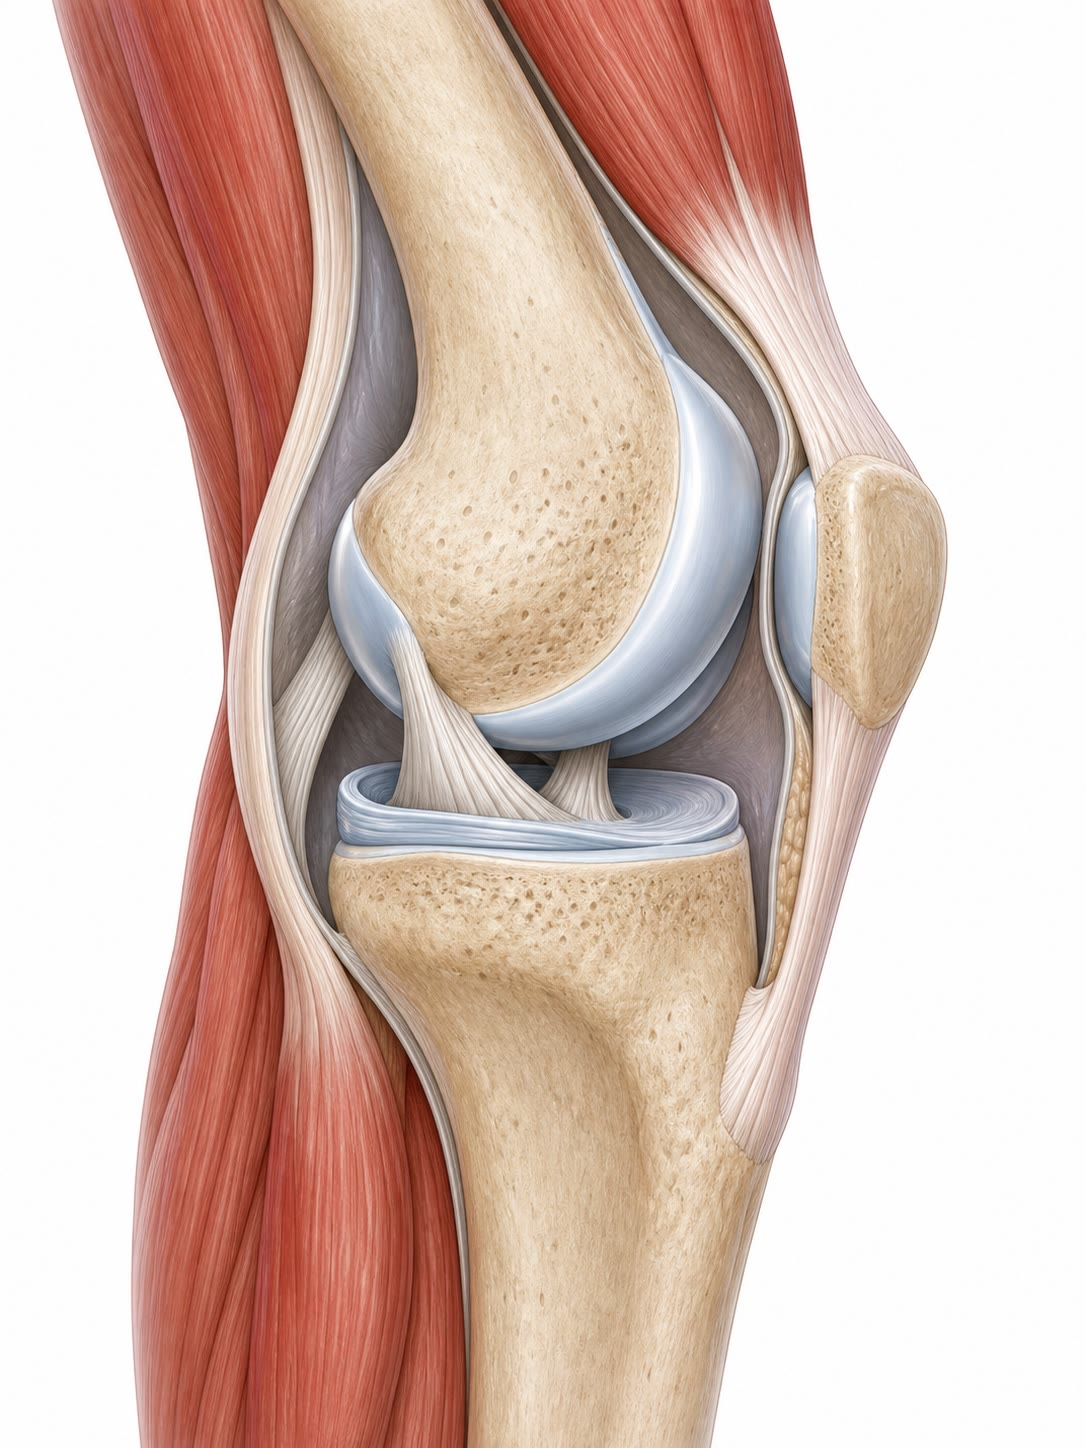
\includegraphics[width=0.4\linewidth]{images/book2/ai/fig-knee-cutaway.jpg}};
  \begin{scope}[x={(img.south east)}, y={(img.north west)},
      every node/.style={font=\small}]
    \draw[omDef, thick] (0.50,0.86) -- (1.05,0.90) node[right] {dijbeen};
    \draw[omDef, thick] (0.76,0.74) -- (1.05,0.74) node[right] {pees van de quadriceps};
    \draw[omDef, thick] (0.82,0.58) -- (1.05,0.58) node[right] {knieschijf};
    \draw[omDef, thick] (0.50,0.20) -- (1.05,0.14) node[right] {scheenbeen};
    \draw[omDef, thick] (0.34,0.60) -- (-0.05,0.64) node[left] {kraakbeen};
    \draw[omDef, thick] (0.50,0.50) -- (-0.05,0.50) node[left] {gewrichtsband};
    \draw[omDef, thick] (0.40,0.44) -- (-0.05,0.36) node[left] {meniscus};
  \end{scope}
\end{tikzpicture}

{\small De knie in doorsnede: het dijbeen boven, het scheenbeen onder, de
knieschijf ervoor in de \omterm{def:g10:muscles-and-joints:muscle}{pees} van de dijspier; \omterm{def:g10:muscles-and-joints:joint}{kraakbeen} op de
boteinden, de meniscus ertussen, \omterm{def:g10:muscles-and-joints:joint}{gewrichtsbanden} die de botten
bijeenhouden.}
\end{omfigure}

\begin{proposition}[Waar elk onderdeel voor dient]\label{prop:g10:muscles-and-joints:parts}
\omterm{def:g10:muscles-and-joints:joint}{Kraakbeen} en gewrichtssmeer laten de oppervlakken met minder wrijving
langs elkaar glijden dan ijs op ijs; de menisci verdelen een belasting
die zich anders op enkele vierkante millimeters zou samenballen; de
\omterm{def:g10:muscles-and-joints:joint}{gewrichtsbanden} laten de knie buigen en strekken maar weerstaan draaien
en zijwaarts buigen; het kapsel houdt de smeer binnen. Elk onderdeel
heeft zijn eigen manier om te bezwijken: \omterm{def:g10:muscles-and-joints:joint}{kraakbeen} slijt (artrose), een
meniscus scheurt bij een draai met gebogen knie, een \omterm{def:g10:muscles-and-joints:joint}{gewrichtsband}
verzwikt of scheurt wanneer het \omterm{def:g10:muscles-and-joints:joint}{gewricht} voorbij zijn bereik wordt
gedwongen.
\end{proposition}
\admitted

\begin{example}[Verzwikking, scheur, ontwrichting]\label{ex:g10:muscles-and-joints:injuries}
Verzwik een enkel op een stoeprand: de \omterm{def:g10:muscles-and-joints:joint}{gewrichtsbanden} aan de buitenkant
worden voorbij hun grens uitgerekt --- een \emph{verzwikking}; het
\omterm{def:g10:muscles-and-joints:joint}{gewricht} zwelt op doordat het kapsel bloedt en er vocht ophoopt. Trek
hard aan een koude hamstring: een deel van haar vezels scheurt --- een
\emph{spierscheur}. Val op een uitgestrekte arm: de kop van het
opperarmbeen kan zijn kom verlaten --- een \emph{ontwrichting}, waarbij
de \omterm{def:g10:muscles-and-joints:joint}{gewrichtsbanden} en het kapsel worden uitgerekt of scheuren. Geen van
alle is een botbreuk; alle kunnen langer duren om te genezen dan een
breuk.
\end{example}

\section{Spieren trekken, en dat in paren}

\begin{definition}[Skeletspier en pees]\label{def:g10:muscles-and-joints:muscle}
Een \emph{skeletspier}\index{skeletspier} is een orgaan dat bestaat uit
duizenden lange \omterm{def:g10:cells-common-unit:cell}{cellen}, de \emph{spiervezels}, in bundels bijeen; elke
vezel wordt korter wanneer een zenuw haar prikkelt. Aan beide uiteinden
versmalt de spier tot een \emph{pees}\index{pees}, een streng
niet-samentrekkend weefsel dat aan bot vastzit. Een spier kan alleen
\emph{trekken}, door korter te worden, en alleen in haar eigen richting:
zij beweegt een \omterm{def:g10:muscles-and-joints:joint}{gewricht} door aan het bot erachter te trekken.
\end{definition}

\begin{proposition}[Antagonistische paren]\label{prop:g10:muscles-and-joints:antagonists}
Omdat een spier niet kan duwen, vergt elke beweging van een \omterm{def:g10:muscles-and-joints:joint}{gewricht} twee
spieren of spiergroepen die tegen elkaar in werken: een \emph{buiger} die
het \omterm{def:g10:muscles-and-joints:joint}{gewricht} buigt en een \emph{strekker} die het strekt. Trekt de ene
samen, dan ontspant de andere en wordt zij uitgerekt; om een houding vast
te houden trekken beide tegelijk samen. De biceps buigt de elleboog en de
triceps strekt hem; de quadriceps aan de voorkant van het dijbeen strekt
de knie, de hamstrings erachter buigen haar.
\end{proposition}
\admitted

\begin{omfigure}
\begin{tikzpicture}[>=Stealth, font=\small, line cap=round]
  % upper arm (humerus) horizontal, forearm angled
  \draw[line width=7pt, gray!45] (0,0) -- (5,0);         % humerus
  \draw[line width=6pt, gray!45] (5,0) -- (8.6,2.0);     % forearm
  \fill[gray!60] (5,0) circle (0.28);
  \node[anchor=north] at (2.5,-0.25) {opperarmbeen};
  \node[anchor=north west] at (7.2,1.1) {onderarm};
  \node[anchor=west] at (5.5,-0.5) {elleboog};
  % biceps: from shoulder region above humerus to forearm just past elbow
  \draw[line width=9pt, omThm!60] (0.6,0.6) .. controls (3,1.4) .. (5.35,0.9);
  \draw[thick, omThm!80!black] (5.35,0.9) -- (5.65,0.45);   % tendon
  \node[omThm!80!black, anchor=south] at (3,1.3) {biceps (buiger): trekt samen};
  % triceps: below humerus to the back of the forearm
  \draw[line width=7pt, omDef!50] (0.6,-0.9) .. controls (3,-1.6) .. (4.9,-1.0);
  \draw[thick, omDef!80!black] (4.9,-1.0) -- (5.25,-0.4);
  \node[omDef!80!black, anchor=north] at (3,-1.65) {triceps (strekker): ontspant, uitgerekt};
  \draw[->, thick] (8.6,2.0) to[bend right=20] (8.0,3.0);
  \node[anchor=south] at (8.3,3.05) {buiging};
  \draw[->, thick, omThm!80!black] (5.65,0.45) -- (5.2,0.75);
\end{tikzpicture}

{\small Een antagonistisch paar bij de elleboog. De biceps, die net
voorbij het \omterm{def:g10:muscles-and-joints:joint}{gewricht} aan de onderarm vastzit, wordt korter en buigt de
elleboog; de triceps, die achter het \omterm{def:g10:muscles-and-joints:joint}{gewricht} vastzit, ontspant en wordt
uitgerekt. Draai de rollen om en de arm strekt zich.}
\end{omfigure}

\begin{proposition}[Hefbomen en krachten]\label{prop:g10:muscles-and-joints:lever}
Een bot dat in een \omterm{def:g10:muscles-and-joints:joint}{gewricht} draait, is een hefboom. De \omterm{def:g10:muscles-and-joints:muscle}{pees} van de spier
zit op een kleine afstand $d$ van het draaipunt vast, terwijl de last op
een grotere afstand $D$ aangrijpt; voor evenwicht moet de spier trekken
met een kracht
\[
F_{\text{spier}} = F_{\text{last}} \times \frac{D}{d},
\]
enkele keren de last. Die opstelling ruilt kracht in voor snelheid en
bereik: een kleine verkorting van de spier levert een grote, snelle
beweging van de hand of de voet op, tegen de prijs van grote krachten in
de \omterm{def:g10:muscles-and-joints:muscle}{pees} en in het \omterm{def:g10:muscles-and-joints:joint}{gewricht}.
\end{proposition}
\admitted

\begin{example}[Een tas vasthouden]\label{ex:g10:muscles-and-joints:bag}
Een tas van \qty{5}{kg} (gewicht \qty{49}{N}) hangt aan de hand, op
\qty{35}{cm} van de elleboog; de peesaanhechting van de biceps zit op
\qty{5}{cm} daarvan. De biceps trekt met $49 \times 35/5 = \qty{343}{N}$
--- zeven keer de last, het gewicht van \qty{35}{kg} --- en het
ellebooggewricht wordt met ongeveer \qty{300}{N} samengedrukt. Spieren,
\omterm{def:g10:muscles-and-joints:muscle}{pezen} en \omterm{def:g10:muscles-and-joints:joint}{kraakbeen} zijn voor die krachten gebouwd; wat hen beschadigt is
een plotselinge kracht in de verkeerde richting, of een belasting die
vaker wordt herhaald dan het weefsel kan herstellen.
\end{example}

\begin{omfigure}
\begin{tikzpicture}[>=Stealth, font=\small]
  \draw[line width=6pt, gray!45] (0,0) -- (7,0);
  \fill[gray!70] (0,0) circle (0.25);
  \node[anchor=north] at (0,-0.35) {elleboog (draaipunt)};
  \draw[->, very thick, omThm] (1,0.15) -- (1,2.2) node[above] {$F_{\text{spier}}$};
  \draw[->, very thick, omDef] (7,-0.15) -- (7,-1.6) node[below] {$F_{\text{last}} = \qty{49}{N}$};
  \draw[<->] (0,0.9) -- (1,0.9) node[midway, above, xshift=-4mm] {$d = \qty{5}{cm}$};
  \draw[<->] (0,-1.25) -- (7,-1.25) node[midway, below] {$D = \qty{35}{cm}$};
\end{tikzpicture}

{\small De onderarm als hefboom: de biceps trekt dicht bij het draaipunt,
de last hangt er ver vandaan. $F_{\text{spier}} \times d =
F_{\text{last}} \times D$, dus is de spierkracht $D/d = 7$ keer de
last.}
\end{omfigure}

\section{Binnen in de spier}

\begin{proposition}[Bouw van een spiervezel]\label{prop:g10:muscles-and-joints:fibre}
Een \omterm{def:g10:muscles-and-joints:muscle}{spiervezel} is één reuzencel, \num{10}--\qty{100}{\micro m} breed en
tot enkele centimeters lang, met vele \omterm{def:g10:cells-common-unit:organelle}{celkernen}. Zij is volgepakt met
evenwijdige \emph{myofibrillen}, elk een keten van zich herhalende
eenheden waarin twee typen eiwitdraden, dikke en dunne, in elkaar
grijpen. Samentrekking is het langs elkaar schuiven van de dunne draden
tussen de dikke, aangedreven door ATP: elke eenheid wordt een fractie
korter, de myofibril met hun som, en de vezel met haar mee. De
\omterm{def:g10:cells-common-unit:organelle}{mitochondriën} tussen de myofibrillen leveren de ATP; een zenuwuiteinde
op elke vezel geeft het bevel.
\end{proposition}
\admitted

\begin{omfigure}
\begin{tikzpicture}[font=\small, >=Stealth]
  \tikzset{lvl/.style={draw, rounded corners, thick, align=center, minimum height=1.1cm}}
  \node[lvl, fill=omThm!12, text width=2.1cm] (m) at (0,0) {spier\\ (orgaan)};
  \node[lvl, fill=omThm!12, text width=2.1cm] (b) at (3.0,0) {bundel\\ vezels};
  \node[lvl, fill=omProp!15, text width=2.1cm] (f) at (6.0,0) {spiervezel\\ (één cel)};
  \node[lvl, fill=omDef!12, text width=2.1cm] (my) at (9.0,0) {myofibril};
  \node[lvl, fill=omMeth!15, text width=2.1cm] (fi) at (12.0,0) {dikke en dunne\\ draden};
  \foreach \a/\b in {m/b, b/f, f/my, my/fi} \draw[->] (\a) -- (\b);
  \node[anchor=north, font=\scriptsize] at (m.south) {centimeters};
  \node[anchor=north, font=\scriptsize] at (b.south) {millimeter};
  \node[anchor=north, font=\scriptsize] at (f.south) {\qty{50}{\micro m} breed};
  \node[anchor=north, font=\scriptsize] at (my.south) {\qty{1}{\micro m} breed};
  \node[anchor=north, font=\scriptsize] at (fi.south) {\qty{10}{nm}};
\end{tikzpicture}

{\small Van de hele spier tot de moleculen die haar korter maken: vijf
ordeningsniveaus, elk een bundel van het volgende. Het langs elkaar
schuiven van de draden, herhaald over elke eenheid, is de samentrekking.}
\end{omfigure}

\begin{definition}[Vezeltypen]\label{def:g10:muscles-and-joints:types}
\omterm{def:g10:muscles-and-joints:muscle}{Spiervezels} komen in twee hoofdtypen voor. \emph{Trage vezels} trekken
langzaam en zwak samen maar zijn onvermoeibaar: rijk aan \omterm{def:g10:cells-common-unit:organelle}{mitochondriën} en
haarvaten, rood door een \omterm{def:g10:chemistry-of-life:families}{eiwit} dat zuurstof vasthoudt, draaien zij op de
ademhaling en overheersen zij in houdingsspieren en bij duursporters.
\emph{Snelle vezels} trekken snel en krachtig samen maar zijn binnen een
minuut moe: armer aan \omterm{def:g10:cells-common-unit:organelle}{mitochondriën}, bleker, steunen zij op de
fosfaatvoorraad en de \omterm{def:g10:cell-metabolism:fermentation}{gisting} en overheersen zij bij sprinters. Het
aandeel in een bepaalde spier is grotendeels erfelijk; training verandert
eerder de omvang en de uitrusting van de vezels dan hun aantal.
\end{definition}

\begin{example}[Een spierbiopt lezen]\label{ex:g10:muscles-and-joints:biopsy}
Een kleuring voor \omterm{def:g10:cell-metabolism:metabolism}{enzymen} van de \omterm{def:g10:cells-common-unit:organelle}{mitochondriën} op een dun plakje
dijspier toont een mozaïek: donkere vezels (traag) en bleke vezels
(snel). Het monster van een marathonloper is voor 80\% donker, dat van
een sprinter voor 30\%, dat van een ongetraind mens ongeveer half om
half. Dezelfde kleuring bij diezelfde loper na een jaar sprinttraining
toont de bleke vezels vergroot, maar niet talrijker.
\end{example}

\section{Vermoeidheid, schade, herstel}

\begin{proposition}[Grenzen van de spier]\label{prop:g10:muscles-and-joints:limits}
Een spier bezwijkt op drie verschillende manieren.
\emph{Vermoeidheid}: de kracht loopt terug wanneer de ATP-aanvoer geen
gelijke tred houdt --- binnen een minuut bij snelle vezels, over uren bij
trage --- en herstelt met rust. \emph{Kramp}: een plotselinge,
aanhoudende, onwillekeurige samentrekking, vaak door uitdroging of
zoutverlies. \emph{Blessure}: vezels die scheuren door een kracht boven
hun sterkte, meestal wanneer de spier koud of moe is, of wordt uitgerekt
terwijl zij samentrekt. Vezels herstellen in weken uit reservecellen in
de spier; een \omterm{def:g10:muscles-and-joints:muscle}{pees} of \omterm{def:g10:muscles-and-joints:joint}{gewrichtsband}, slecht van bloed voorzien, herstelt
in maanden.
\end{proposition}
\admitted

\begin{method}[Een blessure van spier of gewricht analyseren]\label{met:g10:muscles-and-joints:analyse}
\begin{enumerate}
  \item Stel vast welke beweging haar veroorzaakte en in welke richting:
        werd het \omterm{def:g10:muscles-and-joints:joint}{gewricht} binnen zijn bereik bewogen (een spierprobleem)
        of erbuiten (een probleem van \omterm{def:g10:muscles-and-joints:joint}{gewrichtsband} of kapsel)?
  \item Stel het weefsel vast: \omterm{def:g10:muscles-and-joints:muscle}{spiervezels} scheuren (pijn in de buik van
        de spier, krachtverlies); \omterm{def:g10:muscles-and-joints:joint}{gewrichtsbanden} verzwikken (pijn en
        zwelling bij het \omterm{def:g10:muscles-and-joints:joint}{gewricht}, instabiliteit); \omterm{def:g10:muscles-and-joints:muscle}{pezen} ontsteken bij
        herhaalde belasting; \omterm{def:g10:muscles-and-joints:joint}{kraakbeen} slijt in stilte over jaren.
  \item Schat de kracht: gebruik de hefboomregel; bedenk dat landen of
        afremmen het lichaamsgewicht enkele keren vermenigvuldigt.
  \item Voorspel het herstel uit de bloedvoorziening van het weefsel:
        spier in weken, \omterm{def:g10:muscles-and-joints:joint}{gewrichtsband} en \omterm{def:g10:muscles-and-joints:muscle}{pees} in maanden, \omterm{def:g10:muscles-and-joints:joint}{kraakbeen}
        nauwelijks.
\end{enumerate}
\end{method}

\begin{remark}[Waarom opwarmen werkt]\label{rem:g10:muscles-and-joints:warmup}
Tien minuten rustig bewegen verhoogt de temperatuur van de spieren met
een graad of twee, waardoor hun \omterm{def:g10:chemistry-of-life:families}{eiwitten} rekbaarder en hun \omterm{def:g10:cell-metabolism:metabolism}{enzymen}
sneller worden; het opent de haarvaten die de zuurstof uit
\cref{ch:g10:heart-lungs-effort} zullen aanvoeren, en het verdikt het
laagje gewrichtssmeer op het \omterm{def:g10:muscles-and-joints:joint}{kraakbeen}. Een koude spier waarvan een
maximale samentrekking wordt gevraagd, is de gewoonste oorzaak van een
scheur; een \omterm{def:g10:muscles-and-joints:joint}{gewricht} dat wordt belast voordat zijn smeer zich heeft
verspreid, slijt sneller.
\end{remark}

\section{Oefeningen}

\begin{exercise}[$\star$]\label{exo:g10:muscles-and-joints:1}
Noem de onderdelen van een beweeglijk \omterm{def:g10:muscles-and-joints:joint}{gewricht} en geef de rol van elk.
\end{exercise}

\begin{exercise}[$\star$]\label{exo:g10:muscles-and-joints:2}
Wat is het verschil tussen een \omterm{def:g10:muscles-and-joints:muscle}{pees} en een \omterm{def:g10:muscles-and-joints:joint}{gewrichtsband}?
\end{exercise}

\begin{exercise}[$\star$]\label{exo:g10:muscles-and-joints:3}
Waarom heeft elk \omterm{def:g10:muscles-and-joints:joint}{gewricht} ten minste twee spieren nodig om te bewegen?
\end{exercise}

\begin{exercise}[$\star$]\label{exo:g10:muscles-and-joints:4}
Onderscheid een verzwikking, een spierscheur en een ontwrichting naar het
betrokken weefsel.
\end{exercise}

\begin{exercise}[$\star$]\label{exo:g10:muscles-and-joints:5}
Geef twee verschillen tussen trage en snelle \omterm{def:g10:muscles-and-joints:muscle}{spiervezels}.
\end{exercise}

\begin{exercise}[$\star\star$]\label{exo:g10:muscles-and-joints:6}
Een halter van \qty{2}{kg} wordt in de hand gehouden, op \qty{32}{cm} van
de elleboog; de biceps hecht op \qty{4}{cm} daarvan aan. Bereken de
kracht in de biceps ($g = \qty{9.8}{N/kg}$).
\end{exercise}

\begin{exercise}[$\star\star$]\label{exo:g10:muscles-and-joints:7}
Leg uit waarom de biceps en de triceps allebei moeten samentrekken om de
arm stil te houden tegen een onvoorspelbare duw.
\end{exercise}

\begin{exercise}[$\star\star$]\label{exo:g10:muscles-and-joints:8}
Een \omterm{def:g10:muscles-and-joints:muscle}{spiervezel} van \qty{3}{cm} lang wordt bij samentrekking 20\% korter.
Hoeveel beweegt de hand als de \omterm{def:g10:muscles-and-joints:muscle}{pees} van de vezel op \qty{5}{cm} van de
elleboog aanhecht en de hand er \qty{35}{cm} vandaan is?
\end{exercise}

\begin{exercise}[$\star\star$]\label{exo:g10:muscles-and-joints:9}
Waarom is de schouder, het beweeglijkste \omterm{def:g10:muscles-and-joints:joint}{gewricht} van het lichaam, ook
het \omterm{def:g10:muscles-and-joints:joint}{gewricht} dat het vaakst ontwricht?
\end{exercise}

\begin{exercise}[$\star\star$]\label{exo:g10:muscles-and-joints:10}
De kuitspier van een loper krijgt kramp aan het eind van een warme
wedstrijd. Stel twee oorzaken uit het hoofdstuk voor en één remedie.
\end{exercise}

\begin{exercise}[$\star\star$]\label{exo:g10:muscles-and-joints:11}
Leg met \cref{ex:g10:muscles-and-joints:biopsy} uit waarom een sprinter
die voor een marathon traint, minder vooruitgaat dan een ongetraind
iemand van dezelfde leeftijd zou kunnen.
\end{exercise}

\begin{exercise}[$\star\star\star$]\label{exo:g10:muscles-and-joints:12}
Bij het landen na een sprong buigt de knie en draagt de \omterm{def:g10:muscles-and-joints:muscle}{pees} van de
quadriceps ongeveer vier keer het lichaamsgewicht. Bereken die kracht
voor een sporter van \qty{70}{kg}. De \omterm{def:g10:muscles-and-joints:muscle}{pees} heeft een doorsnede van
ongeveer \qty{1}{cm^2} en bezwijkt bij ongeveer \qty{100}{N/mm^2}; hoe
ver zit zij van bezwijken af?
\end{exercise}

\begin{exercise}[$\star\star\star$]\label{exo:g10:muscles-and-joints:13}
Een gescheurde \omterm{def:g10:muscles-and-joints:joint}{gewrichtsband} geneest in maanden, een gescheurde spier in
weken, en beschadigd \omterm{def:g10:muscles-and-joints:joint}{kraakbeen} nauwelijks. Breng die drie in verband met
de bloedvoorziening van de weefsels en met de \omterm{def:g10:cells-common-unit:cell}{cellen} die voor herstel
beschikbaar zijn.
\end{exercise}

\begin{exercise}[$\star\star\star$]\label{exo:g10:muscles-and-joints:14}
Bodybuilding vergroot de spieren; rekken vergroot het bereik van een
\omterm{def:g10:muscles-and-joints:joint}{gewricht}. Welk weefsel verandert elk van beide, en waarom verandert geen
van beide het aantal vezels?
\end{exercise}

\begin{exercise}[$\star\star\star$]\label{exo:g10:muscles-and-joints:15}
Het kniekraakbeen van een oudere is tot de halve dikte gesleten. Leg
vanuit het hoofdstuk uit waarom het \omterm{def:g10:muscles-and-joints:joint}{gewricht} pijn doet op de trap,
waarom de menisci belangrijker zijn dan vroeger, en waarom de spieren
rond de knie deel uitmaken van de behandeling.
\end{exercise}

\section{Probleem: De krachten in een knie}

\begin{problem}[{Weekendprobleem --- de knie van een voetballer uit
elkaar gehaald: de hefboom van het been, de trek van de dijspier, de
gewrichtsband die scheurde, en de getallen die een pees bij elke stap
draagt}]
\label{pb:g10:muscles-and-joints:1}
Karim, \qty{70}{kg}, blesseerde zijn knie door scherp te draaien op een
vaststaande voet. Neem $g = \qty{9.8}{N/kg}$. De \omterm{def:g10:muscles-and-joints:muscle}{pees} van de quadriceps
hecht op \qty{5}{cm} van het draaipunt van de knie aan het scheenbeen
aan; de duw van de grond op de voet grijpt aan op ongeveer \qty{20}{cm}
daarvan wanneer de knie flink gebogen is, zoals bij een landing.

\medskip
\noindent\textbf{Deel I --- Staan en stappen.}
\begin{enumerate}
  \item Bereken het gewicht van Karim.
  \item Bij het staan op één been met licht gebogen knie duwt de grond
        met zijn hele gewicht omhoog tegen de voet, aangrijpend op
        \qty{10}{cm} van het draaipunt van de knie. Bereken de kracht in
        de \omterm{def:g10:muscles-and-joints:muscle}{pees} van de quadriceps.
  \item Bij het beklimmen van een trap is de knie verder gebogen en
        grijpt de grondkracht aan op \qty{20}{cm} van het draaipunt.
        Bereken de peeskracht opnieuw.
  \item Druk de twee uitkomsten uit als veelvouden van het
        lichaamsgewicht, en leg uit waarom trappen de dijen vermoeien.
  \item Welke spiergroep is de antagonist van de quadriceps, en wat doet
        zij tijdens de stap?
\end{enumerate}

\medskip
\noindent\textbf{Deel II --- De landing.}
\begin{enumerate}[resume]
  \item Bij het landen na een kopbal duwt de grond met drie keer het
        gewicht van Karim, op \qty{20}{cm} van het draaipunt. Bereken de
        peeskracht.
  \item De doorsnede van de \omterm{def:g10:muscles-and-joints:muscle}{pees} is \qty{1.2}{cm^2}. Bereken de spanning
        erin, in newton per vierkante millimeter, en vergelijk met de
        breukspanning van ongeveer \qty{100}{N/mm^2}.
  \item De gewrichtsoppervlakken worden samengedrukt met ongeveer de
        peeskracht plus de grondkracht. Bereken die belasting, en
        vervolgens de druk op het \omterm{def:g10:muscles-and-joints:joint}{kraakbeen} als het contactoppervlak
        \qty{6}{cm^2} is met de menisci en \qty{1}{cm^2} zonder.
  \item Leid daaruit af waarom een knie die een meniscus heeft verloren,
        haar \omterm{def:g10:muscles-and-joints:joint}{kraakbeen} sneller slijt.
  \item Leg uit wat de gewrichtssmeer tijdens de landing bijdraagt.
\end{enumerate}

\medskip
\noindent\textbf{Deel III --- De blessure.}
\begin{enumerate}[resume]
  \item De voet van Karim stond vast en zijn lichaam draaide: welke
        bewegingsrichting werd de knie opgelegd, en welk weefsel is
        gebouwd om die te weerstaan?
  \item Waarom beschermde de quadriceps, die met enkele kilonewton kan
        trekken, de \omterm{def:g10:muscles-and-joints:joint}{gewrichtsband} niet?
  \item De knie zwol binnen een uur op. Wat vulde haar, en welk deel van
        het \omterm{def:g10:muscles-and-joints:joint}{gewricht} was doorbroken?
  \item Een scan toont een gescheurde \omterm{def:g10:muscles-and-joints:joint}{gewrichtsband} en een gescheurde
        meniscus. Voorspel met
        \cref{met:g10:muscles-and-joints:analyse} de hersteltijd van elk
        en verantwoord dat vanuit hun bloedvoorziening.
  \item Karim vraagt waarom de chirurg zijn hamstrings vóór de operatie
        wil versterken. Antwoord met
        \cref{prop:g10:muscles-and-joints:antagonists}.
\end{enumerate}

\medskip
\noindent\textbf{Deel IV --- Elke stap telt.}
\begin{enumerate}[resume]
  \item Karim zet ongeveer 8000 stappen per dag; de helft op het geblesseerde
        been. Hoe vaak per dag draagt de \omterm{def:g10:muscles-and-joints:muscle}{pees} met de kracht uit vraag 2
        ten minste die belasting?
  \item Wat is het totale aantal belastingen over een jaar? Leg uit
        waarom een \omterm{def:g10:muscles-and-joints:muscle}{pees} die door overbelasting ontstoken is
        (peesontsteking) rust nodig heeft in plaats van kracht.
  \item Tijdens een wedstrijd landt hij zo'n 40 keer na een sprong.
        Vergelijk de totale belasting bij de landingen (vraag 6) met die
        bij de stappen van de dag.
  \item Hardlopen verdubbelt de grondkracht ten opzichte van wandelen.
        Waarom raden artsen bij een genezende knie fietsen en zwemmen aan
        in plaats van hardlopen?
  \item Geef het resultaat: het veelvoud van het lichaamsgewicht dat de
        \omterm{def:g10:muscles-and-joints:muscle}{pees} van de quadriceps op een trap en bij een landing draagt, en
        het ene weefsel van de knie waarvan die getallen de sterkte nooit
        beproefden --- tot aan de draai.
\end{enumerate}
\end{problem}
